\section{Fonctionnalités}
\label{s:fonctionnalités}

\subsection{Image}
\subsubsection{Exportation d'image}
Il est possible d'exporter des rendus de la scène dans des fichiers PNG.
Pour ce faire, il suffit d'appuyer sur la barre espace et une capture d'écran de la fenêtre de l'application est sauvegardée dans le dossier \textit{/bin/data}.
Le fichier image est nommé en fonction de la date et de l'heure selon le format y$-$m$-$d\_hms.png.

\begin{figure}[H]
    \centering
	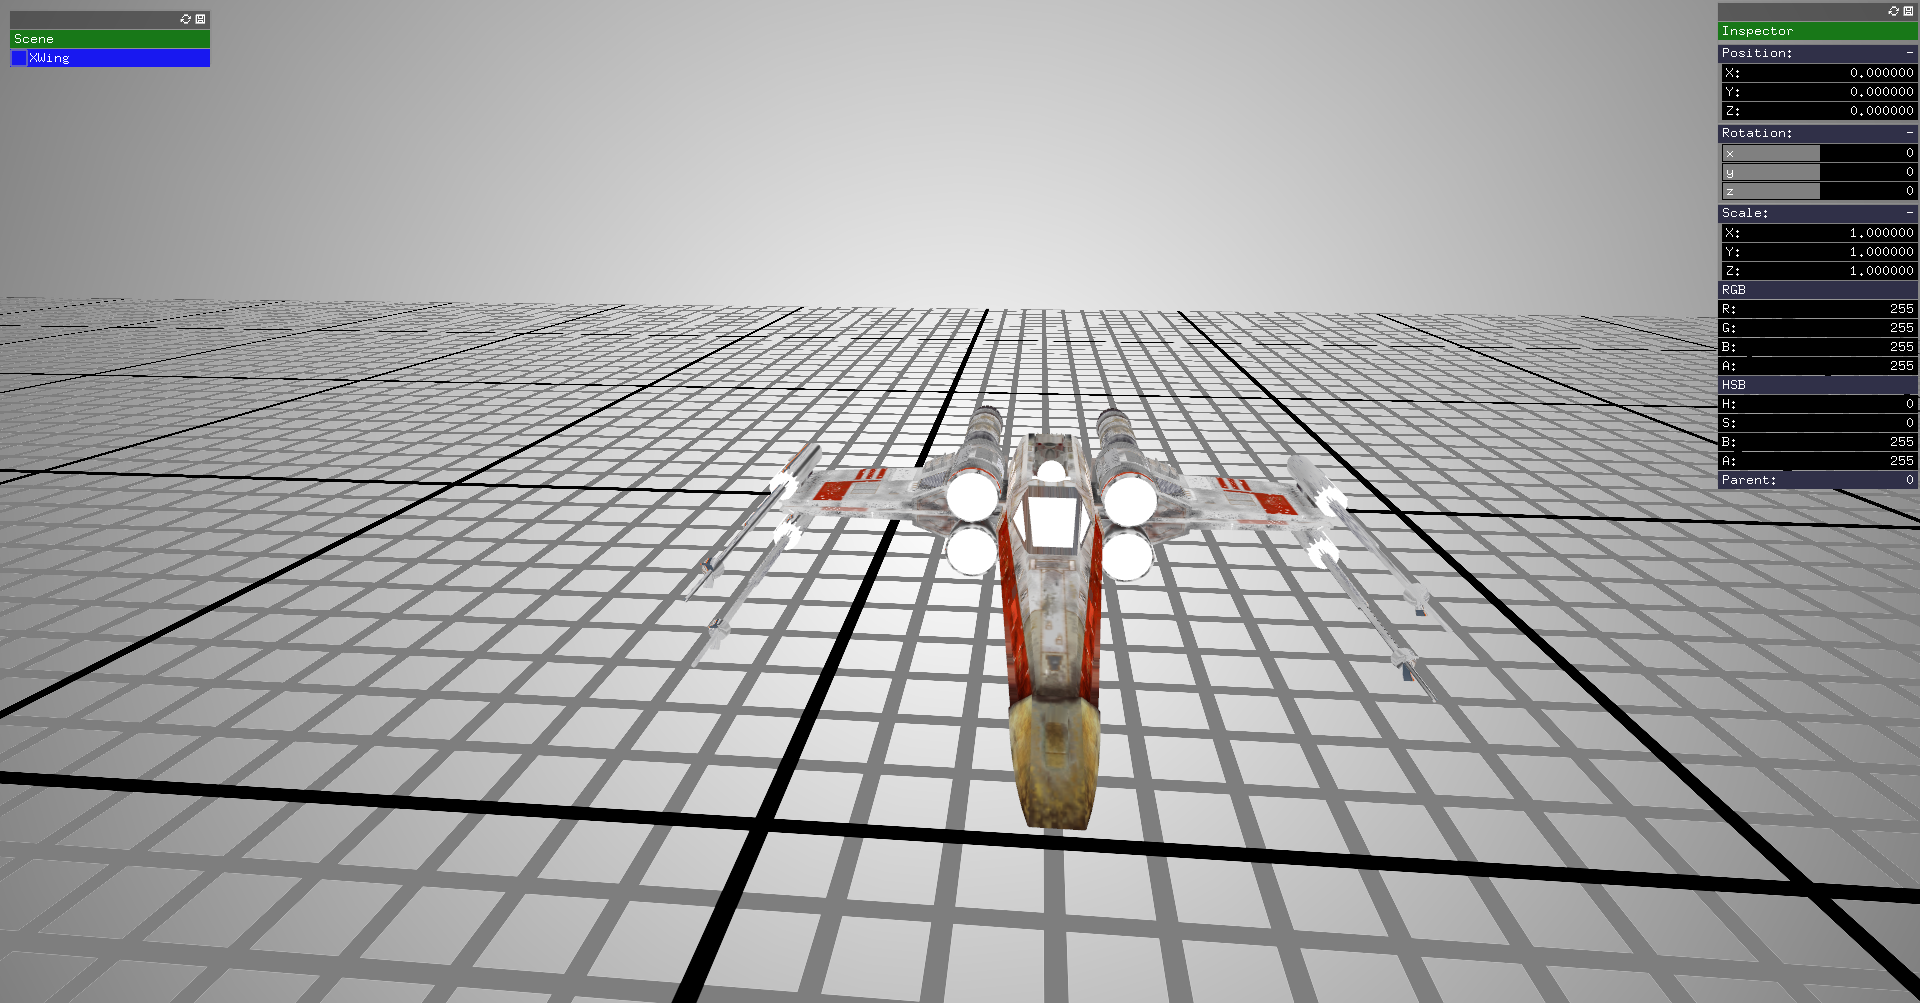
\includegraphics[scale=0.1]{fig/2018-3-11_22h34m38s.png}
	\caption{Exemple de capture d'écran}
	\label{fig:capture_ecran}
\end{figure}

\begin{figure}[H]
    \centering
	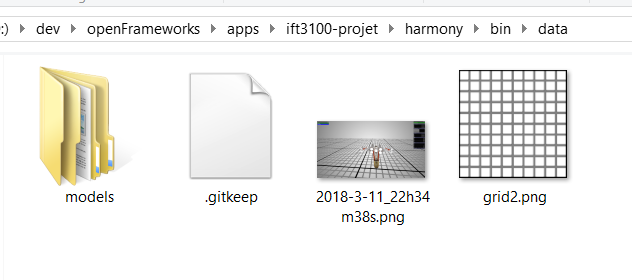
\includegraphics[scale=0.5]{fig/preuve-capture.png}
	\caption{Fichier exporté}
	\label{fig:preuve-capture}
\end{figure}

L'algorithme de capture d'écran est le suivant:
\begin{figure}[H]
    \centering
	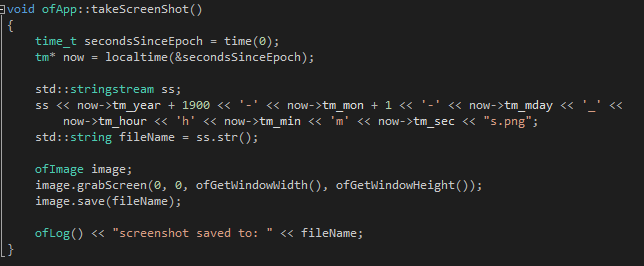
\includegraphics[scale=0.5]{fig/screenshotducodequiprenddesscreenshots.PNG}
	\caption{Code de la capture d'écran}
	\label{fig:capture_ecran}
\end{figure}

\subsubsection{Sélecteur de couleur}
\label{ss:selecteur_de_couleur}
L'inspecteur offre deux sélecteurs de couleurs affichant les valeurs des composantes de couleur de l'objet sélectionné et permettant de les modifier.
Chaque composante de couleur est encodée sur 8 bits, ce qui signifie que les sélecteurs acceptent des entiers entre 0 et 255.
\begin{figure}[H]
    \centering
	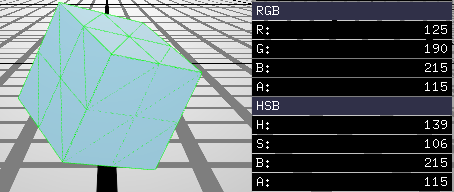
\includegraphics[scale=0.8]{fig/couleur.PNG}
	\caption{Sélecteurs de couleur}
	\label{fig:color_picker}
\end{figure}
Lorsque l'utilisateur entre une valeur dans un des champs, on récupère chacune des composantes et on applique cette couleurs à chaque vertex de l'objet sélectionné.

\subsubsection{Espace de couleur}
Un des sélecteurs de couleur de l'inspecteur permet de travailler en espace RGBA alors que l'autre permet de travailler en espace HSBA (voir la figure \ref{fig:color_picker}).
Lorsque la valeur d'une composante est modifiée dans un espace de couleur, l'autre sélecteur est mis à jour afin d'afficher les valeurs correspondantes.


\subsection{Dessin vectoriel}
\subsubsection{Primitives vectorielles}
\subsubsection{Forme vectorielle}
\subsubsection{Interface}

\subsection{Transformation}
\subsubsection{Graphe de scène}
\subsubsection{Transformations interactives}
\subsubsection{Historique des transformations}
\paragraph{} L'historique de transformation permet d'annuler et de récupérer une action provenant de l'utilisateur. Pour l'application, il est possible d'avoir l'historique du déplacement, de la rotation, de l'échelle et de la couleur pour chaque objet avec les touches \texttt{Ctrl+Z} et \texttt{Ctrl+Y}.
\paragraph{} L'état d'un objet \texttt{GameObject} est sauvegardé dans une classe \texttt{Command} à chacunes de ces actions. Le nombre de sauvegarde de commande est limité à 500. Cette commande est gérée par la classe \texttt{CommandHandler} qui s'occupe de sauvegarder les états courants (\texttt{CommandHandler::add()}), d'appliquer les changements d'état (\texttt{CommandHandler::undo()/redo()}) et d'ordonner les commandes dans deux \texttt{std::stack} dont une pour récupérer les commandes et une autre pour les annuler. Cette classe appartient à la classe \texttt{Scene} qui appelle la méthode de sauvegarde d'état à chaque fonction de modification d'un \texttt{GameObject}. Elle offre aussi les méthodes \texttt{Scene::undo()} et \texttt{Scene::redo()} pour que les événements puissent contrôler l'historique des transformations.

\subsection{Géométrie}
\subsubsection{Boîte de délimitation}
\subsubsection{Primitives géométriques}
\subsubsection{Modèle 3D}

\subsection{Texture}
\subsubsection{Mapping}
\subsubsection{Texture procédurale}
\paragraph{} Les textures procédurales proviennent d'un patron de base sur lequel est appliqué des algorithmes. Les patrons de bases utilisés sont le bruit de perlin, le patron en sinus et le patron en cercle.
\paragraph{} Il est possible de générer une texture procédurale imitant l'effet nuage avec le bruit de perlin, une interpolation linéaire, un algorithme de turbulence et une modification les paramètres HSL. L'effet marbre est généré par le patron en sinus sur lequel on applique un algorithme de turbulence. L'effet bois est généré par le patron en cercle sur lequel on applique un algorithme de turbulence ainsi qu'un filtre de couleur bois (orangé / brun).
\begin{figure}[H]
\centering
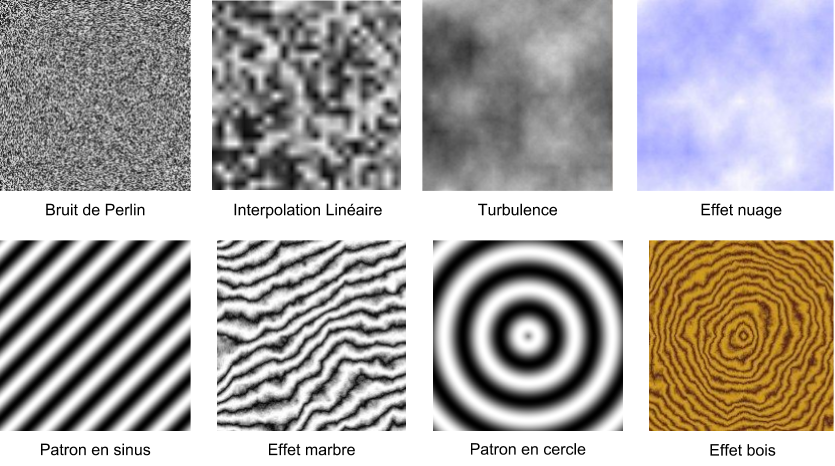
\includegraphics[width=\textwidth]{img/infog-image-procedural-texture.png}
\caption{Textures procédurales}\label{fig-procedural-texture}
\end{figure}
\paragraph{} Au niveau de l'application, une classe \texttt{texelFactory} s'occupe de générer toutes les textures procédurales présentées plus-haut (\ref{fig-procedural-texture}).  Chaque textue est interfacée par une méthode permettant de transformer un buffer \texttt{ofPixels} avec des paramètres (puissance de la turbulence par exemple) qui seront utilisées par les algorithmes correspondants (réf. \ref{src-procedural-texture}). Par la suite, ce buffer est appliqué sur le \texttt{GameObject} qui possède un \texttt{ofTexture} et un \texttt{ofMesh} propre. Aussi, lors de la création du \texttt{ofMesh}, il est nécessaire de cartographier la texture sur la forme avec la méthode \texttt{ofMesh::addTextCoord} et \texttt{ofTexture::getCoordFromPercent}.
\subsubsection{Cubemap}